% Einf�hrungskapitel
%

\chapter{Introduction}

In 2014, the Neurorobotics team of the Blue Brain Project (BBP), project of the Ecole Federale Polytechnique Federale de Lausanne (EPFL), successfully produced a point-neuron model
of a mouse brain from data provided by the Allen Institute for Brain Science (Provide reference of Allen Institute).
Using NEST software, the BBP Neurorobotics team was then able to simulate a
scaled-down model of the mouse brain on a laptop computer, paving the way towards
making a mouse brain interact with an environment. A full-scale implementation of
the mouse brain model is possible, but requires the of large scale resources with low latency requirements only modern supercomputers can today provide.
The current functionality of NEST supports  generating large neuronal networks
on a super computer based an random distributions but not yet from experimental data contained in brain atlases. 
We suggest as part of this thesis to first develop the means to fully model a mouse brain from experimental data using NEST software on available supercomputing architectures.
\newpage

\section{Brain Simulations}
\section{Anatomy of the brain}
 
 The human brain is the main part of the central nervous system
 which consists of the spinal cord, sensory organs
 and all of the nerves that connect these organs with the rest of the body.
 These organs are responsible for the control of the body and communication between its parts.
 The nervous system is the most complex system of our body with respect to functionality.
 It contains billions of nerve and glia cells. 
 The nerve cells are connected via synapses to a complex network.
 Electrical pulses from neuron to neuron transmit information through the network.
 Glia cells help to maintain the right concentration of chemical substances in the
 extracellular space around neurons and provide supporting structures for the
 growth of neurons and for their spatial arrangement.
  \subsection{Macroscopic structure}
  \label{sec:Macroscopicstructure}
  The anatomy of the brain as depicted in Figure \ref{Aufbau1}, shows that different parts vary in cell density and functionality.
 Figure \ref{Aufbau1} shows a cross-section of the human brain. The outer layer is called the gray matter, due to the color caused by the high density of nerve cells.
 The white matter, which is underneath the gray matter,
 consists most of connection fibers of the nerve cells.
 The thalamus is situated in the middle of the brain and functions as a relay station between the sensory system and the cortical systems for cognition and motor control.
  \begin{figure}[!htbp]
  \subfigure[A cross-section of the human brain shows different densities of nerve cells \cite{CN}.]{
  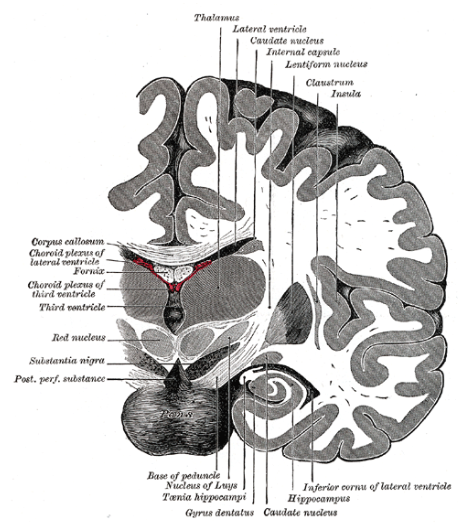
\includegraphics[scale=0.3]{pictures/Aufbau1.png}
  \label{Aufbau1}
  }
  \hfill
  \subfigure[A general map of the human brain assigns parts of the gray matter to fuctionalities \cite{CN}.]{
  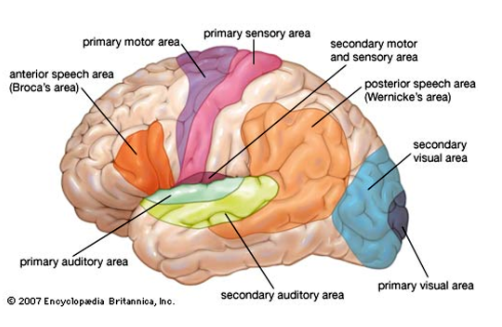
\includegraphics[scale=0.3]{pictures/Aufbau2.png}
  \label{Aufbau2}
  }
  \hfill
  \subfigure[The vertical structure of the gray matter shows six layers \cite{CN}.]{
  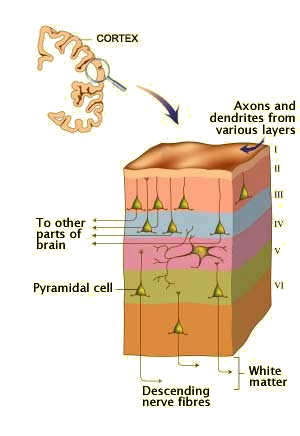
\includegraphics[scale=0.3]{pictures/mikro_aufbau.png}
  \label{mikroaufbau}
  }
  \caption{The macroscopic structure of the human brain.}
  \end{figure}
  Because of the high density of nerve cells the gray matter is the main part of information processing of the brain.
  
  The number of nerve cells (neurons), the number of connections (synapses) and the structure differs from person to person.
  The connections of each neuron are dynamic and change over time.
  Some parts of the brain can still be assigned roughly to functionality as shown in Figure \ref{Aufbau2}.\\
  Having a look at the vertical structure of the cortex,
  the gray matter can be partitioned in six layers as shown in figure \ref{mikroaufbau}.
  The cells in each layer have similarities like cell type, connections to other layers and connections to the thalamus and other parts.
  %-forebrain(anterior part of the brain)
  %-neocortex(surface of the mammalian brain, gray)
 
 
  \newpage
  \subsection{Microscopic structure}
  The nerve cells are tiny structures which are connected to each other.
  For an understanding of the brain a deeper look at the nerve cells is necessary.
  There are different cell types in a brain. They vary in structure and size.
  Pyramidal, spiny stellate and smooth stellate cells occur most often.
  For each layer there are types which occur more frequent. 
  
  In Figure \ref{Corticalneurons} a typical neuron is depicted.
  It contains the soma (the cell body) dendrites and axons.
  Electrical pulses are transported from the dendrites to the soma.
  In case of a spike an electrical impulse is forwarded through the axon.
  These axons are connected via synapses to further dendrites.
  The electrical impulse is transmitted via a chemical reaction in the synapse to the dendrites of connected cells.
  \begin{figure}[!htbp]
    \centering
    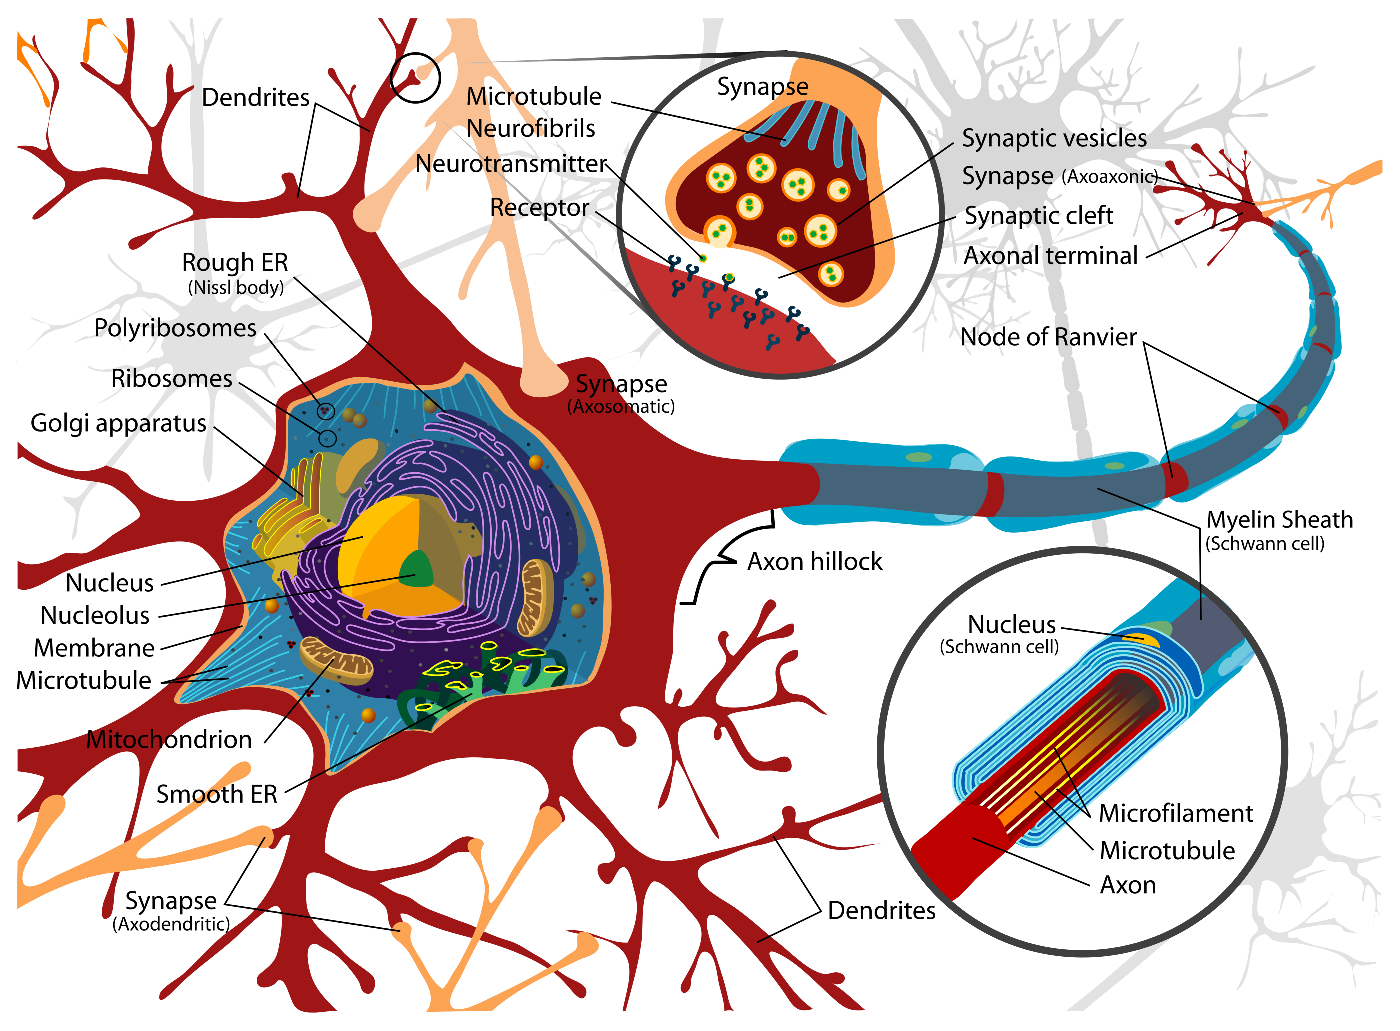
\includegraphics[scale=0.65]{pictures/Complete_neuron_cell_diagram_en.eps}
    \caption{Microscopic structure of a neuron. \cite{neuronpic}}
    \label{Corticalneurons}
  \end{figure}
  There are excitatory and inhibitory neurons.
  The excitatory neurons excite the following neurons, 
  in contrast the inhibitory neurons inhibit the following neurons.
  Via electrical currents the connected neurons influence the membrane potential of each neuron.
  The membrane potential can be measured.
  As an example the membrane potential is plotted over time in Figure \ref{membrane_potential}.
  Chemical processes inside the neuron generate a spike if the membrane potential reaches a specific electrical level called the threshold.  
  As shown in Figure \ref{membrane_potential} spikes are peaks in the membrane potential.  
  
  %-cortical neurons
  %-different cells: pyramidal, spiny stellate, smooth stellate
  %-cortical layers
  %-synapses
  
  %-10e12 neurons in the human brain
  \newpage
  \begin{figure}[!htbp]
  \subfigure[The plot shows the membrane potential of a neuron over the time.
  The peaks are called spikes.
  There are four spikes in the time span shown.
  The firing threshold of the cell is at about 58 mV \cite{CN}.]{
  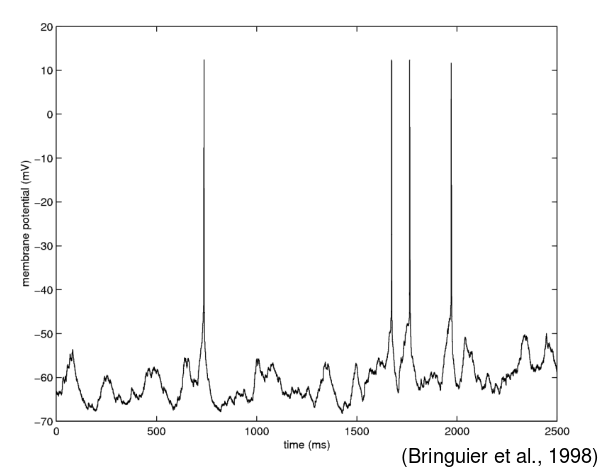
\includegraphics[scale=0.36]{pictures/membrane_potential.png}
  \label{membrane_potential}
  }
  \hfill
  \subfigure[The dot plot shows spikes of each neuron over time. On the y-axis there are the neurons number.
  The histogram in the lower panel sums up all spikes for each time bin. \cite{CN}]{
  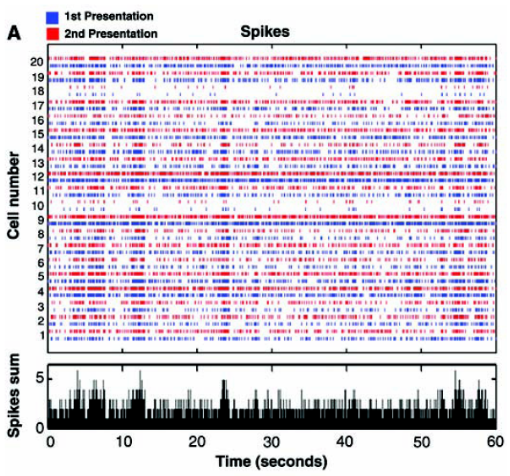
\includegraphics[scale=0.36]{pictures/spike_plot.png}
  \label{spikeplot}
  }
  \caption{The activity of a single neurons is displayed using its membrane potential. For multiple neurons the information is reduced to spike timings.}
  \end{figure}
  
  In order to analyze the membrane potential more objectively it is reduced to timings of the spikes.
  For multiple neuron the spike timings in a dot plot can be visualized as in Figure \ref{spikeplot}.
  One can get an overview of the activity in a whole neuronal network if the spike sums are
  plotted (summed up spikes for each time bin) in a so-called histogram.

	\begin{itemize}
      \item Short overview over simulators: NEST, NEURON, STEPS
      \item Possibilities/limits of simulations
   \end{itemize}
   
\section{Virtual mouse}
	\begin{itemize}
      \item Available data
      \item Why of interest
   	\end{itemize}   
\newpage
\section{Allen Brain Atlas}
   Allen Institute for Brain Science provides a high-resolution map of neural connections in the mouse brain.
   It contains several injection experiments. The provided datasets of the experiments 
   contain a 3D image of the injection and a 3D image of its axonal projection labeled by viral
   tracers.
   
   \begin{figure}[ht!]
   	\begin{center}
        \subfigure[Injection sites - showing all available experiments]{%
            \label{fig:allInjections}
            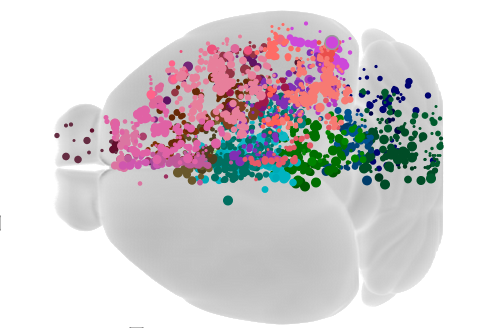
\includegraphics[width=0.4\textwidth]{pictures/connectionBrowser_allinjections.png}
        }
        \hspace{1cm}
        \subfigure[Projection density of one experiment]{%
            \label{fig:oneProjection}
            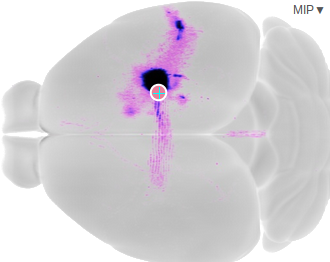
\includegraphics[width=0.32\textwidth]{pictures/connectionBrowser_oneinjections.png}
       }
    	   \end{center}
    	\caption{%
        The pictures are inverted and copied from the Allen Brain Atlas.
     }%
   \label{fig:atlas}
   \end{figure}
   
   \begin{itemize}
      \item description
\end{itemize}
   
\section{BBP recipe}
\begin{figure}[ht!]
\centering
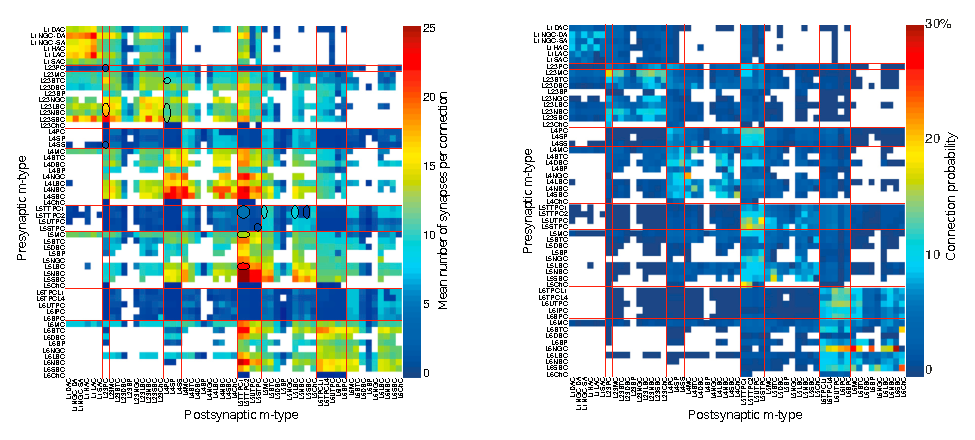
\includegraphics[scale=0.9]{pictures/BBPconnectionPropasMatrix.eps}
\end{figure}

\begin{itemize}
      \item description
\end{itemize}

\section{NEST}
NEST is a simulator for spiking neural network models that focuses on the dynamics, size and structure of neural systems rather than on the exact morphology of individual neurons. The development of NEST is coordinated by the NEST Initiative. NEST is ideal for networks of spiking neurons of any size, for example:
Models of information processing e.g. in the visual or auditory cortex of mammals, models of network activity dynamics, e.g. laminar cortical networks or balanced random networks and models of learning and plasticity. A NEST simulation tries to follow the logic of an electrophysiological experiment that takes place inside a computer with the difference, that the neural system to be investigated must be defined by the experimenter. The definition is based on number of neurons with parameters and connections between these neurons. NEST supports the generation based on probabilistic values. The stochastic settings of a neuronal network can be used to create its artificial copy inside of NEST. To manipulate or observe the network dynamics, the experimenter can define so-called devices which represent the various instruments (for measuring and stimulation) found in an experiment. These devices write their data either to memory or to file. 

\section{Visualization}
To interpret the output of a neuronal simulation the spiking activity of the neurons is analyzed, mostly. 
Different types of methods allow to extract stochastic characteristics from spike trains.
Besides this visualization of the spike trains taking their location into account,
can give an impression of the activity.

\begin{itemize}
      \item Visualization tools available
      \item BBP
      \item ViSNEST
\end{itemize}
